\documentclass[12pt]{article}
 
\usepackage[margin=0.8in]{geometry}
\usepackage{amsmath}
\usepackage{amssymb}
\usepackage{graphicx}
\usepackage{tikz}
\usepackage{pgfplots}

\pgfplotsset{compat=1.18}

\title{Precalculus: Functions and Their Graphs - Homework}
\author{Student Name: \_\_\_\_\_\_\_\_\_\_\_\_\_\_\_\_\_\_\_\_}
\date{\today}

\begin{document}

\maketitle

\section*{Instructions}
Solve the following problems. Show all your work and explain your reasoning where appropriate. Use additional paper if needed.

\begin{enumerate}

\item Find the equation of the line passing through the points (1, 4) and (3, 8). Express your answer in slope-intercept form.

\vspace{3cm}

\item Given $f(x) = x^2 - 2x + 3$ and $g(x) = x + 1$, find:
\begin{itemize}
    \item[(a)] $(f \circ g)(x)$
    \item[(b)] $(g \circ f)(x)$
    \item[(c)] Evaluate $(f \circ g)(2)$
\end{itemize}

\vspace{5cm}

\item Starting with the function $f(x) = |x|$, graph $g(x) = |x - 1| + 2$. Describe all transformations applied to $f(x)$ to get $g(x)$.

\vspace{2cm}

\begin{center}
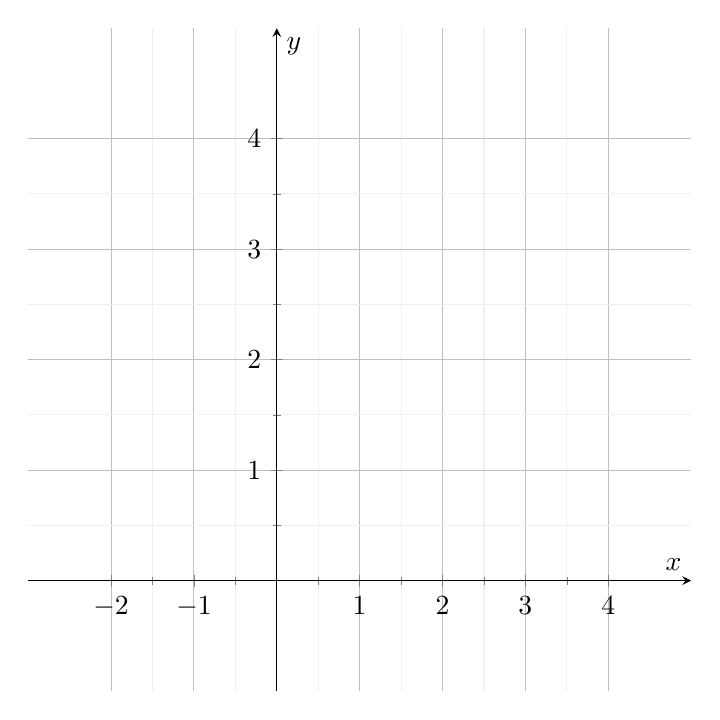
\begin{tikzpicture}
\begin{axis}[
    axis lines = middle,
    xlabel = $x$,
    ylabel = $y$,
    xmin = -3, xmax = 5,
    ymin = -1, ymax = 5,
    xtick = {-2,-1,0,1,2,3,4},
    ytick = {0,1,2,3,4},
    grid = both,
    minor tick num = 1,
    major grid style = {lightgray},
    minor grid style = {lightgray!25},
    width = 10cm,
    height = 10cm,
]
\end{axis}
\end{tikzpicture}
\end{center}

\item Let $f(x) = x^2 + 1$ and $g(x) = 2x - 3$.
\begin{itemize}
    \item[(a)] Find an expression for $(f + g)(x)$
    \item[(b)] Find an expression for $(f \cdot g)(x)$
    \item[(c)] Evaluate $(f + g)(3)$ and $(f \cdot g)(3)$
\end{itemize}

\vspace{5cm}

\item Find the inverse function for $f(x) = 3x + 4$. Then, find $f^{-1}(10)$.

\vspace{4cm}

\item For the function $h(x) = x^2 - 4x - 5$:
\begin{itemize}
    \item[(a)] Find the y-intercept
    \item[(b)] Find the x-intercepts
    \item[(c)] Find the vertex of the parabola
    \item[(d)] Is the parabola opening upward or downward?
\end{itemize}

\vspace{6cm}

\item Given the function $f(x) = \frac{x + 2}{x - 1}$:
\begin{itemize}
    \item[(a)] Find the domain of $f(x)$
    \item[(b)] Find any vertical and horizontal asymptotes
    \item[(c)] Sketch the graph of $f(x)$
\end{itemize}

\vspace{2cm}

\begin{center}
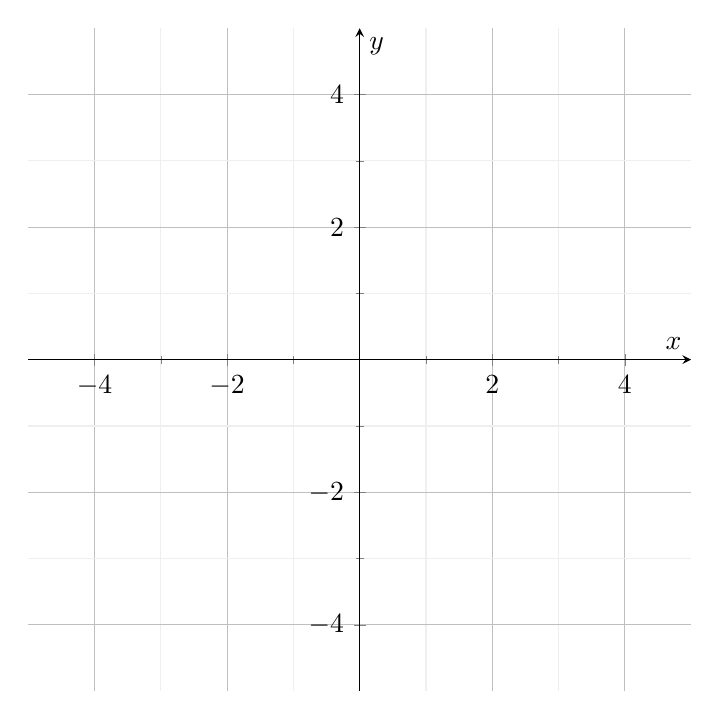
\begin{tikzpicture}
\begin{axis}[
    axis lines = middle,
    xlabel = $x$,
    ylabel = $y$,
    xmin = -5, xmax = 5,
    ymin = -5, ymax = 5,
    xtick = {-4,-2,0,2,4},
    ytick = {-4,-2,0,2,4},
    grid = both,
    minor tick num = 1,
    major grid style = {lightgray},
    minor grid style = {lightgray!25},
    width = 10cm,
    height = 10cm,
]
\end{axis}
\end{tikzpicture}
\end{center}

\item Determine if the function $f(x) = x^3 - x$ is one-to-one. Explain your reasoning.

\vspace{4cm}

\item Find the domain and range of the function $f(x) = \sqrt{x + 2}$. Then, sketch its graph.

\vspace{2cm}

\begin{center}
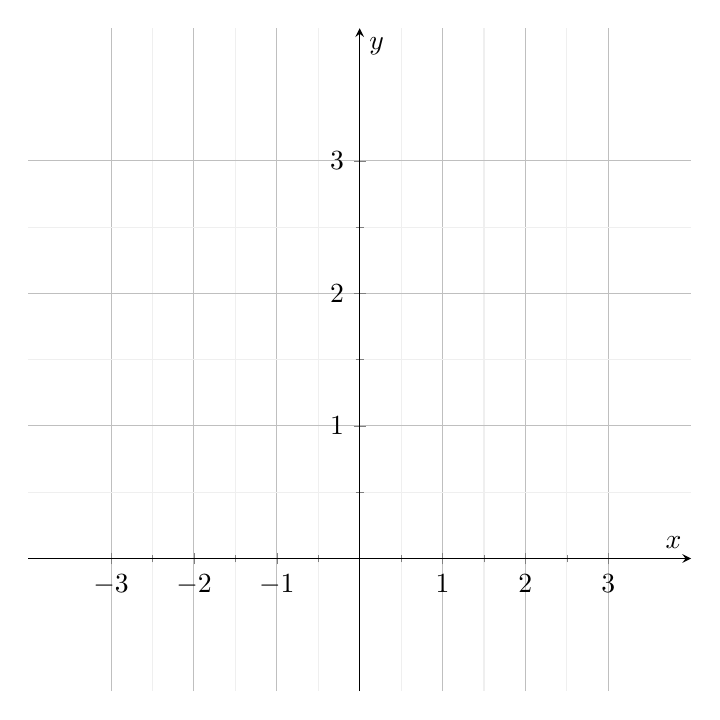
\begin{tikzpicture}
\begin{axis}[
    axis lines = middle,
    xlabel = $x$,
    ylabel = $y$,
    xmin = -4, xmax = 4,
    ymin = -1, ymax = 4,
    xtick = {-3,-2,-1,0,1,2,3},
    ytick = {0,1,2,3},
    grid = both,
    minor tick num = 1,
    major grid style = {lightgray},
    minor grid style = {lightgray!25},
    width = 10cm,
    height = 10cm,
]
\end{axis}
\end{tikzpicture}
\end{center}

\item For the function $f(x) = 2^x$, find and graph $g(x) = 2^{x+1} - 1$. Describe all transformations applied to $f(x)$ to get $g(x)$.

\vspace{2cm}

\begin{center}
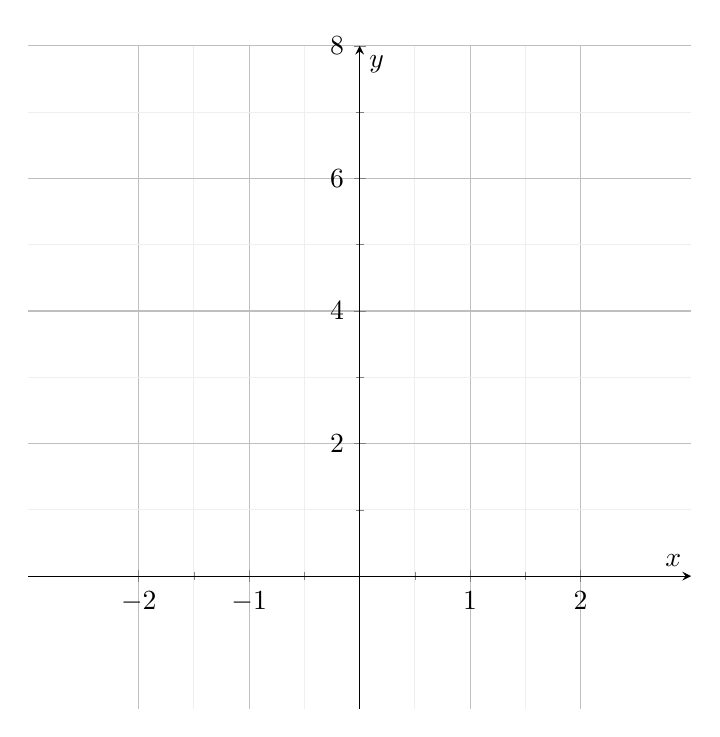
\begin{tikzpicture}
\begin{axis}[
    axis lines = middle,
    xlabel = $x$,
    ylabel = $y$,
    xmin = -3, xmax = 3,
    ymin = -2, ymax = 8,
    xtick = {-2,-1,0,1,2},
    ytick = {0,2,4,6,8},
    grid = both,
    minor tick num = 1,
    major grid style = {lightgray},
    minor grid style = {lightgray!25},
    width = 10cm,
    height = 10cm,
]
\end{axis}
\end{tikzpicture}
\end{center}

\item Solve the equation: $\log_2(x + 3) = 4$

\vspace{3cm}

\item Find the x-coordinate(s) of the point(s) where the graphs of $y = x^2 - 2x - 3$ and $y = 2x + 1$ intersect.

\vspace{4cm}

\item Given $f(x) = 3x - 1$ and $g(x) = \frac{x}{2} + 1$, find $(f \circ g)(x)$ and $(g \circ f)(x)$.

\vspace{4cm}

\item Sketch the graph of $y = |x^2 - 4|$. Identify any key features (intercepts, vertex, etc.).

\vspace{2cm}

\begin{center}
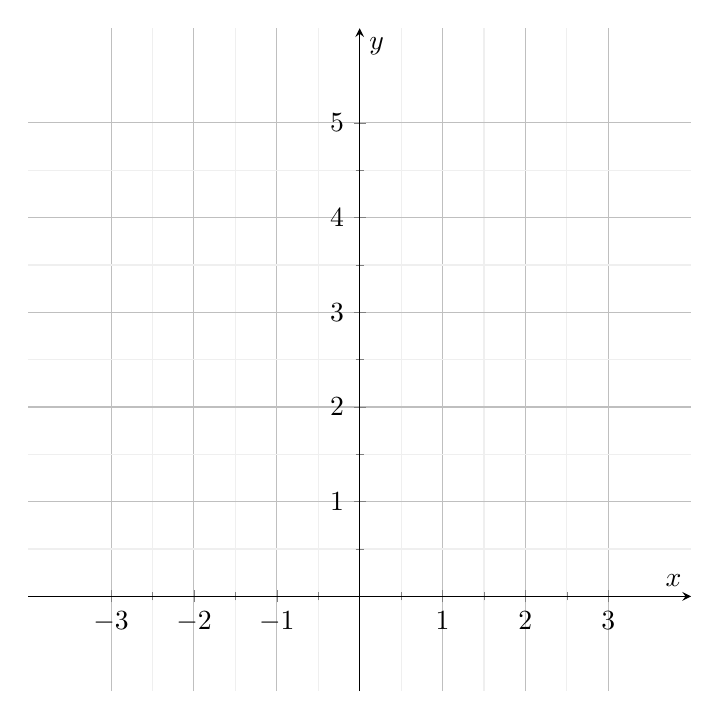
\begin{tikzpicture}
\begin{axis}[
    axis lines = middle,
    xlabel = $x$,
    ylabel = $y$,
    xmin = -4, xmax = 4,
    ymin = -1, ymax = 6,
    xtick = {-3,-2,-1,0,1,2,3},
    ytick = {0,1,2,3,4,5},
    grid = both,
    minor tick num = 1,
    major grid style = {lightgray},
    minor grid style = {lightgray!25},
    width = 10cm,
    height = 10cm,
]
\end{axis}
\end{tikzpicture}
\end{center}

\item For the function $f(x) = \frac{1}{x-2}$, describe how its graph relates to the graph of $y = \frac{1}{x}$. What transformations have been applied?

\vspace{3cm}

\end{enumerate}

\end{document}